% !TeX root = ../main.tex
\section{Additional Results}
\label{app:additional-results}

This appendix reports the complete factor-level result ledger and the full
robustness summaries used in the main text. Percentages are reported to two
decimal places. $A_S$ is measured on the independent static set; $A_B$ is
unconditioned accuracy on the RewardLens-CLEVR base images; RA and II are
conditional on a correct base decision.

\FloatBarrier

\subsection{All Model--Factor Measurements}
\label{app:all-model-factor-results}

Table~\ref{tab:all_32_results} contains every one of the $8\times4=32$
model--factor measurements. Each factor has 200 frozen static items and 200
frozen audit triplets. All static estimates use 200 reported outcomes except
Phi-3.5-Vision on Spatial ($n=198$); no imputation is used. The conditional
denominator $n_B$ is the number of base-correct audit triplets for that model
and factor.

\begin{table*}[t]
\centering
\scriptsize
\caption{Complete model--factor ledger. Each cell is $A_S$/RA/II in percent;
the corresponding audit-base denominators are reported in
Table~\ref{tab:all_32_base_accuracy}. All $A_S$ estimates use $n=200$ except
Phi-3.5-Vision on Spatial ($n=198$; marked $^{\dagger}$); no imputation is used.}
\label{tab:all_32_results}
\setlength{\tabcolsep}{3.2pt}
\begin{tabular}{lrrrrrrrrrrrr}
\toprule
& \multicolumn{3}{c}{Count} & \multicolumn{3}{c}{Attribute}
& \multicolumn{3}{c}{Presence} & \multicolumn{3}{c}{Spatial} \\
Judge & $A_S$ & RA & II & $A_S$ & RA & II & $A_S$ & RA & II & $A_S$ & RA & II \\
\midrule
Qwen3-VL-4B & 91.50 & 17.00 & 100.00 & 82.00 & 100.00 & 100.00 & 89.50 & 100.00 & 100.00 & 80.00 & 98.50 & 100.00 \\
Gemma-3-4B & 38.50 & 32.41 & 87.59 & 72.50 & 95.19 & 97.33 & 75.00 & 60.10 & 100.00 & 56.00 & 0.00 & 97.95 \\
Molmo-7B-D & 62.50 & 18.63 & 97.06 & 67.00 & 98.96 & 98.96 & 79.50 & 74.37 & 98.99 & 66.00 & 39.86 & 99.32 \\
Skywork-VL-Reward-7B & 76.00 & 62.81 & 98.99 & 93.00 & 100.00 & 100.00 & 84.50 & 100.00 & 98.49 & 84.50 & 86.00 & 100.00 \\
Idefics3-8B & 81.50 & 71.43 & 95.77 & 76.50 & 100.00 & 100.00 & 79.00 & 100.00 & 99.50 & 64.00 & 55.00 & 100.00 \\
Phi-3.5-Vision & 63.50 & 20.00 & 95.15 & 80.50 & 84.95 & 89.25 & 92.00 & 73.89 & 97.22 & $84.85^{\dagger}$ & 47.40 & 98.44 \\
LLaVA-OneVision-7B & 78.50 & 42.08 & 98.91 & 80.50 & 100.00 & 100.00 & 88.50 & 98.00 & 100.00 & 78.50 & 87.00 & 100.00 \\
InternVL3-8B & 69.00 & 18.00 & 100.00 & 85.50 & 100.00 & 100.00 & 80.00 & 100.00 & 100.00 & 68.50 & 91.50 & 100.00 \\
\bottomrule
\end{tabular}
\end{table*}

\begin{table}[t]
\centering
\scriptsize
\caption{Complete $|\Delta A_S|\leq1$ pp matched-pair census. All gaps are
absolute percentage points.}
\label{tab:matched_pairs_1pp}
\begin{tabular}{llrrr}
\toprule
Factor & Pair & $\Delta A_S$ & $\Delta\mathrm{RA}$ & $\Delta\mathrm{II}$\\
\midrule
Spatial & Skywork--Phi & .35 & 38.60 & 1.56\\
Presence & Molmo--Idefics3 & .50 & 25.63 & .51\\
Presence & Molmo--InternVL & .50 & 25.63 & 1.01\\
Attribute & Phi--LLaVA & .00 & 15.05 & 10.75\\
Presence & Qwen--LLaVA & 1.00 & 2.00 & .00\\
Count & Molmo--Phi & 1.00 & 1.37 & 1.91\\
Presence & Idefics3--InternVL & 1.00 & .00 & .50\\
\bottomrule
\end{tabular}
\end{table}

\begin{table*}[t]
\centering
\scriptsize
\caption{Audit-base accuracy and conditional denominators for the same 32
measurements in Table~\ref{tab:all_32_results}. Each entry is $A_B$ (\%) / $n_B$.}
\label{tab:all_32_base_accuracy}
\setlength{\tabcolsep}{7pt}
\begin{tabular}{lrrrr}
\toprule
Judge & Count & Attribute & Presence & Spatial \\
\midrule
Qwen3-VL-4B & 100.0 / 200 & 100.0 / 200 & 99.5 / 199 & 100.0 / 200 \\
Gemma-3-4B & 72.5 / 145 & 93.5 / 187 & 99.0 / 198 & 73.0 / 146 \\
Molmo-7B-D & 51.0 / 102 & 96.5 / 193 & 99.5 / 199 & 74.0 / 148 \\
Skywork-VL-Reward-7B & 99.5 / 199 & 100.0 / 200 & 99.5 / 199 & 100.0 / 200 \\
Idefics3-8B & 94.5 / 189 & 100.0 / 200 & 100.0 / 200 & 100.0 / 200 \\
Phi-3.5-Vision & 82.5 / 165 & 93.0 / 186 & 90.0 / 180 & 96.0 / 192 \\
LLaVA-OneVision-7B & 91.5 / 183 & 100.0 / 200 & 100.0 / 200 & 100.0 / 200 \\
InternVL3-8B & 100.0 / 200 & 100.0 / 200 & 100.0 / 200 & 100.0 / 200 \\
\bottomrule
\end{tabular}
\end{table*}

\subsection{Full Robustness Tables}
\label{app:robustness-tables}

\paragraph{Paired bootstrap.}
For each primary matched pair, we resample matched source triplets jointly for
the two judges ($10{,}000$ replicates; seed 20270915). Table~\ref{tab:paired-bootstrap}
reports signed model-A minus model-B contrasts, so its sign depends on the
printed order. Static contrasts are resampled on shared static item identifiers;
the reported static point estimate can therefore differ slightly from the
displayed difference between separately rounded static percentages.

\begin{table*}[t]
\centering
\scriptsize
\caption{Paired-bootstrap contrasts for all primary matched pairs (percentage
points; 95\% percentile intervals). All audit contrasts resample 200 matched
source triplets jointly across the two judges.}
\label{tab:paired-bootstrap}
\setlength{\tabcolsep}{4pt}
\begin{tabular}{llrrr}
\toprule
Factor & Ordered comparison & Static $\Delta$ [95\% CI] & RA $\Delta$ [95\% CI] & II $\Delta$ [95\% CI] \\
\midrule
Spatial & Skywork $-$ Phi & $-0.51$ [$-6.06$, 5.05] & 38.60 [29.78, 47.23] & 1.56 [0.00, 3.61] \\
Attribute & Phi $-$ LLaVA & 0.00 [$-5.50$, 5.50] & $-15.05$ [$-20.43$, $-10.21$] & $-10.75$ [$-15.46$, $-6.42$] \\
Presence & Molmo $-$ Idefics3 & 0.50 [$-6.50$, 7.50] & $-25.63$ [$-31.66$, $-19.60$] & $-0.51$ [$-2.04$, 1.00] \\
Presence & Molmo $-$ InternVL & $-0.50$ [$-6.00$, 5.50] & $-25.63$ [$-31.82$, $-19.60$] & $-1.01$ [$-2.53$, 0.00] \\
Count & Molmo $-$ Phi & $-1.00$ [$-6.50$, 4.50] & $-1.37$ [$-10.23$, 7.55] & 1.91 [$-2.68$, 6.40] \\
Presence & Qwen $-$ LLaVA & 1.00 [$-3.00$, 5.00] & 2.00 [0.50, 4.00] & 0.00 [0.00, 0.00] \\
Presence & Idefics3 $-$ InternVL & $-1.00$ [$-7.00$, 5.00] & 0.00 [0.00, 0.00] & $-0.50$ [$-1.50$, 0.00] \\
\bottomrule
\end{tabular}
\end{table*}

\paragraph{Shared-base-correct support.}
Table~\ref{tab:shared-base-correct-full} recomputes RA and II on the
intersection of the two judges' base-correct sets. It is a common-support
diagnostic, not a replacement for the judge-conditional definitions in
Eqs.~\ref{eq:emp_ra}--\ref{eq:emp_ii}.

\begin{table*}[t]
\centering
\scriptsize
\caption{All seven primary matched pairs on shared base-correct support.
Entries show model-A/model-B percentages; gaps are absolute percentage points.}
\label{tab:shared-base-correct-full}
\setlength{\tabcolsep}{5pt}
\begin{tabular}{llrrrrr}
\toprule
Factor & Pair & $n_{\cap}$ & RA A/B & $|\Delta\mathrm{RA}|$ & II A/B & $|\Delta\mathrm{II}|$ \\
\midrule
Spatial & Skywork--Phi & 192 & 86.98 / 47.40 & 39.58 & 100.00 / 98.44 & 1.56 \\
Presence & Molmo--Idefics3 & 199 & 74.37 / 100.00 & 25.63 & 98.99 / 99.50 & 0.50 \\
Presence & Molmo--InternVL & 199 & 74.37 / 100.00 & 25.63 & 98.99 / 100.00 & 1.01 \\
Attribute & Phi--LLaVA & 186 & 84.95 / 100.00 & 15.05 & 89.25 / 100.00 & 10.75 \\
Count & Molmo--Phi & 100 & 17.00 / 4.00 & 13.00 & 99.00 / 100.00 & 1.00 \\
Presence & Qwen--LLaVA & 199 & 100.00 / 97.99 & 2.01 & 100.00 / 100.00 & 0.00 \\
Presence & Idefics3--InternVL & 200 & 100.00 / 100.00 & 0.00 & 99.50 / 100.00 & 0.50 \\
\bottomrule
\end{tabular}
\end{table*}

\begin{table}[t]
\centering
\scriptsize
\caption{Sensitivity to the within-factor static-matching
tolerance. All gaps are absolute percentage points.}
\label{tab:threshold-sensitivity-full}
\begin{tabular}{rrrrrr}
\toprule
Tolerance & Pairs & Median RA & 90th RA & Max RA & RA $\geq10$ pp \\
\midrule
1 pp & 7 & 15.05 & 30.82 & 38.60 & 4 \\
2 pp & 11 & 15.05 & 25.63 & 38.60 & 7 \\
3 pp & 15 & 15.14 & 34.90 & 51.64 & 11 \\
\bottomrule
\end{tabular}
\end{table}

\begin{table}[t]
\centering
\scriptsize
\caption{Image-level edit diagnostics by factor. Pixel-change fraction and
global SSIM are computed after resizing to 256 pixels; SSIM is a global RGB
statistic, not a semantic mask measurement.}
\label{tab:edit-magnitude-full}
\begin{tabular}{lrrrr}
\toprule
& \multicolumn{2}{c}{Pixel-change fraction} & \multicolumn{2}{c}{Global SSIM} \\
Factor & Relevant & Irrelevant & Relevant & Irrelevant \\
\midrule
Count & 0.229 & 0.229 & 0.925 & 0.922 \\
Attribute & 0.118 & 0.179 & 0.974 & 0.958 \\
Presence & 0.175 & 0.201 & 0.935 & 0.918 \\
Spatial & 0.375 & 0.265 & 0.817 & 0.890 \\
\bottomrule
\end{tabular}
\end{table}

As an additional post-hoc sensitivity analysis, the magnitude-matched subset
retains 459 of 800 triplets under
$\lvert p_R-p_I\rvert\leq0.05$: 191 Count, 109 Attribute, 103 Presence, and
56 Spatial triplets. On the 109 retained Attribute triplets, Phi is
base-correct on 101 and has RA $=83.17\%$; LLaVA has RA $=100.00\%$.
This is an approximately 16.8 percentage-point RA gap on that restricted
subset.

\subsection{Representative Frozen Audit Triplets}
\label{app:qualitative-triplets}

Figure~\ref{fig:representative-triplets} shows one retained PASS triplet per
factor. These are direct copies of frozen renders; no scene was regenerated or
manually edited for the manuscript. Count changes or preserves the target-color
count; Attribute recolors the target or a matched non-target; Presence removes
the queried conjunction or a matched non-target; and Spatial moves the queried
referent or a matched distractor.

\begin{figure*}[t]
\centering
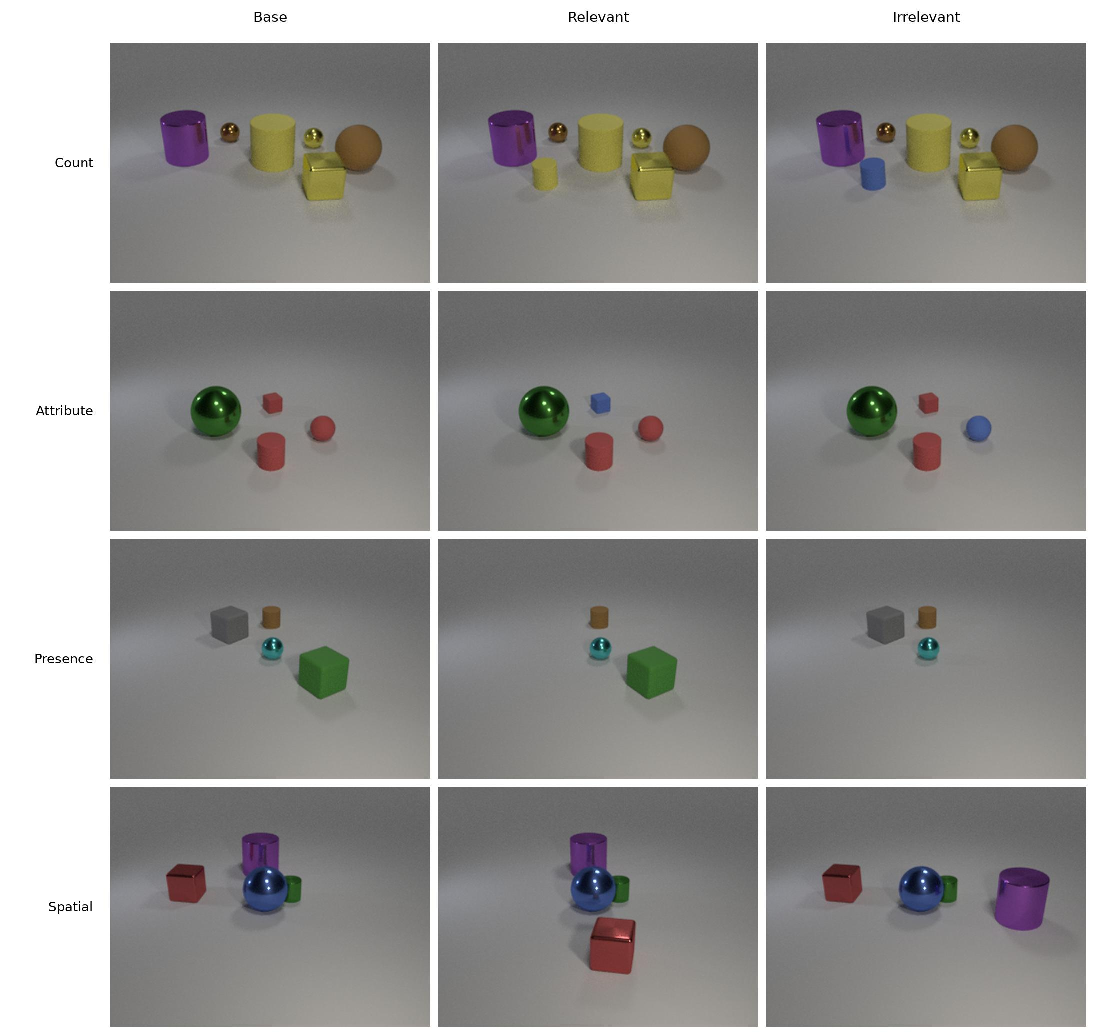
\includegraphics[width=.98\textwidth]{figures/representative_triplets.pdf}
\caption{Representative frozen RewardLens-CLEVR PASS triplets. Columns are
Base, Relevant, and Irrelevant. Rows respectively illustrate target-category
count change versus a matched non-target count change; target versus non-target
recoloring; queried-conjunction versus matched non-target removal; and queried
referent versus matched distractor translation. The source triplet identifiers
are Count \texttt{count\_000000}, Attribute \texttt{attr\_000000}, Presence
\texttt{pres\_000000}, and Spatial \texttt{spat\_000000}.}
\label{fig:representative-triplets}
\end{figure*}
